%%%%%%%%%%%%%%%%%%%%%%%%%%%%%%%%%%%%%%%%%
% Lachaise Assignment
% LaTeX Template
% Version 1.0 (26/6/2018)
%
% This template originates from:
% http://www.LaTeXTemplates.com
%
% Authors:
% Marion Lachaise & François Févotte
% Vel (vel@LaTeXTemplates.com)
%
% License:
% CC BY-NC-SA 3.0 (http://creativecommons.org/licenses/by-nc-sa/3.0/)
% 
%%%%%%%%%%%%%%%%%%%%%%%%%%%%%%%%%%%%%%%%%

%----------------------------------------------------------------------------------------
%	PACKAGES AND OTHER DOCUMENT CONFIGURATIONS
%----------------------------------------------------------------------------------------

\documentclass{article}

%%%%%%%%%%%%%%%%%%%%%%%%%%%%%%%%%%%%%%%%%
% Lachaise Assignment
% Structure Specification File
% Version 1.0 (26/6/2018)
%
% This template originates from:
% http://www.LaTeXTemplates.com
%
% Authors:
% Marion Lachaise & François Févotte
% Vel (vel@LaTeXTemplates.com)
%
% License:
% CC BY-NC-SA 3.0 (http://creativecommons.org/licenses/by-nc-sa/3.0/)
% 
%%%%%%%%%%%%%%%%%%%%%%%%%%%%%%%%%%%%%%%%%

%----------------------------------------------------------------------------------------
%	PACKAGES AND OTHER DOCUMENT CONFIGURATIONS
%----------------------------------------------------------------------------------------

\usepackage{amsmath,amsfonts,stmaryrd,amssymb} % Math packages
\usepackage[dvipsnames]{xcolor}
\usepackage{enumerate} % Custom item numbers for enumerations
\usepackage{hyperref}
\usepackage[ruled,vlined]{algorithm2e} % Algorithms

\usepackage[framemethod=tikz]{mdframed} % Allows defining custom boxed/framed environments

\usepackage{listings} % Required for insertion of code

\newcommand{\randomcolor}{%
  \definecolor{randomcolor}{RGB}
   {
    \pdfuniformdeviate 256,
    \pdfuniformdeviate 256,
    \pdfuniformdeviate 256
   }%
  \color{randomcolor}%
}

\definecolor{codegreen}{rgb}{0,0.6,0}
\definecolor{codegray}{rgb}{0.5,0.5,0.5}
\definecolor{codepurple}{rgb}{0.58,0,0.82}
\definecolor{backcolour}{rgb}{1,1,1}
\lstdefinestyle{mystyle}{
    backgroundcolor=\color{backcolour},   
    commentstyle=\color{codegreen},
    keywordstyle=\color{magenta},
    numberstyle=\tiny\color{codegray},
    stringstyle=\color{codepurple},
    basicstyle=\ttfamily\footnotesize,
    breakatwhitespace=false,         
    breaklines=true,                 
    captionpos=b,                    
    keepspaces=true,                 
    numbers=left,                    
    numbersep=5pt,                  
    showspaces=false,                
    showstringspaces=false,
    showtabs=false,                  
    tabsize=2
}
\renewcommand{\lstlistingname}{Código}% Listing -> Algorithm
\lstset{style=mystyle}


%\usepackage{listings} % File listings, with syntax highlighting
%\lstset{
%	basicstyle=\ttfamily, % Typeset listings in monospace font
%}

%----------------------------------------------------------------------------------------
%	DOCUMENT MARGINS
%----------------------------------------------------------------------------------------

\usepackage{geometry} % Required for adjusting page dimensions and margins

\geometry{
	paper=a4paper, % Paper size, change to letterpaper for US letter size
	top=2.5cm, % Top margin
	bottom=3cm, % Bottom margin
	left=2.5cm, % Left margin
	right=2.5cm, % Right margin
	headheight=14pt, % Header height
	footskip=1.5cm, % Space from the bottom margin to the baseline of the footer
	headsep=1.2cm, % Space from the top margin to the baseline of the header
	%showframe, % Uncomment to show how the type block is set on the page
}

%----------------------------------------------------------------------------------------
%	FONTS
%----------------------------------------------------------------------------------------

\usepackage[utf8]{inputenc} % Required for inputting international characters
\usepackage[T1]{fontenc} % Output font encoding for international characters

\usepackage{XCharter} % Use the XCharter fonts
\usepackage{pgfplots}
\usepackage{multicol}
%----------------------------------------------------------------------------------------
%	COMMAND LINE ENVIRONMENT
%----------------------------------------------------------------------------------------

% Usage:
% \begin{commandline}
%	\begin{verbatim}
%		$ ls
%		
%		Applications	Desktop	...
%	\end{verbatim}
% \end{commandline}

\mdfdefinestyle{commandline}{
	leftmargin=10pt,
	rightmargin=10pt,
	innerleftmargin=15pt,
	middlelinecolor=black!50!white,
	middlelinewidth=2pt,
	frametitlerule=false,
	backgroundcolor=black!5!white,
	frametitle={Command Line},
	frametitlefont={\normalfont\sffamily\color{white}\hspace{-1em}},
	frametitlebackgroundcolor=black!50!white,
	nobreak,
}

% Define a custom environment for command-line snapshots
\newenvironment{commandline}{
	\medskip
	\begin{mdframed}[style=commandline]
}{
	\end{mdframed}
	\medskip
}

%----------------------------------------------------------------------------------------
%	FILE CONTENTS ENVIRONMENT
%----------------------------------------------------------------------------------------

% Usage:
% \begin{file}[optional filename, defaults to "File"]
%	File contents, for example, with a listings environment
% \end{file}

\mdfdefinestyle{file}{
	innertopmargin=1.6\baselineskip,
	innerbottommargin=0.8\baselineskip,
	topline=false, bottomline=false,
	leftline=false, rightline=false,
	leftmargin=2cm,
	rightmargin=2cm,
	singleextra={%
		\draw[fill=black!10!white](P)++(0,-1.2em)rectangle(P-|O);
		\node[anchor=north west]
		at(P-|O){\ttfamily\mdfilename};
		%
		\def\l{3em}
		\draw(O-|P)++(-\l,0)--++(\l,\l)--(P)--(P-|O)--(O)--cycle;
		\draw(O-|P)++(-\l,0)--++(0,\l)--++(\l,0);
	},
	nobreak,
}

% Define a custom environment for file contents
\newenvironment{file}[1][File]{ % Set the default filename to "File"
	\medskip
	\newcommand{\mdfilename}{#1}
	\begin{mdframed}[style=file]
}{
	\end{mdframed}
	\medskip
}

%----------------------------------------------------------------------------------------
%	NUMBERED QUESTIONS ENVIRONMENT
%----------------------------------------------------------------------------------------

% Usage:
% \begin{question}[optional title]
%	Question contents
% \end{question}

\mdfdefinestyle{question}{
	innertopmargin=1.2\baselineskip,
	innerbottommargin=0.8\baselineskip,
	roundcorner=5pt,
	nobreak,
	singleextra={%
		\draw(P-|O)node[xshift=1em,anchor=west,fill=white,draw,rounded corners=5pt]{%
		Pregunta \theQuestion\questionTitle};
	},
}

\newcounter{Question} % Stores the current question number that gets iterated with each new question

% Define a custom environment for numbered questions
\newenvironment{question}[1][\unskip]{
	\bigskip
	\stepcounter{Question}
	\newcommand{\questionTitle}{~#1}
	\begin{mdframed}[style=question]
}{
	\end{mdframed}
	\medskip
}

%----------------------------------------------------------------------------------------
%	WARNING TEXT ENVIRONMENT
%----------------------------------------------------------------------------------------

% Usage:
% \begin{warn}[optional title, defaults to "Warning:"]
%	Contents
% \end{warn}

\mdfdefinestyle{warning}{
	topline=false, bottomline=false,
	leftline=false, rightline=false,
	nobreak,
	singleextra={%
		\draw(P-|O)++(-0.5em,0)node(tmp1){};
		\draw(P-|O)++(0.5em,0)node(tmp2){};
		\fill[black,rotate around={45:(P-|O)}](tmp1)rectangle(tmp2);
		\node at(P-|O){\color{white}\scriptsize\bf !};
		\draw[very thick](P-|O)++(0,-1em)--(O);%--(O-|P);
	}
}

% Define a custom environment for warning text
\newenvironment{warn}[1][Warning:]{ % Set the default warning to "Warning:"
	\medskip
	\begin{mdframed}[style=warning]
		\noindent{\textbf{#1}}
}{
	\end{mdframed}
}

%----------------------------------------------------------------------------------------
%	INFORMATION ENVIRONMENT
%----------------------------------------------------------------------------------------

% Usage:
% \begin{info}[optional title, defaults to "Info:"]
% 	contents
% 	\end{info}

\mdfdefinestyle{info}{%
	topline=false, bottomline=false,
	leftline=false, rightline=false,
	nobreak,
	singleextra={%
		\fill[black](P-|O)circle[radius=0.4em];
		\node at(P-|O){\color{white}\scriptsize\bf i};
		\draw[very thick](P-|O)++(0,-0.8em)--(O);%--(O-|P);
	}
}

% Define a custom environment for information
\newenvironment{info}[1][Info:]{ % Set the default title to "Info:"
	\medskip
	\begin{mdframed}[style=info]
		\noindent{\textbf{#1}}
}{
	\end{mdframed}
}
 % Include the file specifying the document structure and custom commands

%----------------------------------------------------------------------------------------
%	ASSIGNMENT INFORMATION
%----------------------------------------------------------------------------------------

\title{ITC-ADA-C1-2023: Assignment \#5} % Title of the assignment

\author{Luis Ballado\\ \texttt{luis.ballado@cinvestav.mx}} % Author name and email address

\date{CINVESTAV UNIDAD TAMAULIPAS --- \today} % University, school and/or department name(s) and a date

%----------------------------------------------------------------------------------------

\begin{document}

\maketitle % Print the title

%----------------------------------------------------------------------------------------
%	INTRODUCTION
%----------------------------------------------------------------------------------------

%--- cambiar estilo de secciones
\titleformat{\section}  % which section command to format
  {\fontsize{12}{12}\bfseries} % format for whole line
  {\thesection} % how to show number
  {1em} % space between number and text
  {} % formatting for just the text
  [] % formatting for after the text

\section{Diseñe e implemente los algoritmos necesarios para resolver eficientemente los dos incisos del problema 4.13 de la página 127 del libro de Dasgupta, Papadimitriou y Vazirani. Analice matemáticamente la complejidad temporal de sus algoritmos.}

\begin{question}
  \textbf{Dado un conjunto de ciudades, junto con el patrón de carreteras entre ellas, en forma de un gráfico no dirigido G=(V,E). Cada tramo de la carretera $e \in E$ conecta dos de las ciudades, y usted conoce su longitud en millas. Suponga que quiere ir de la ciudad $s$ a la ciudad $t$ . Pero hay un problema, su coche solo puede contener suficiente gasolina para cubrir L millas. Hay gasolineras en cada ciudad, pero no entre ciudades. Por lo tanto, solo se puede tomar una ruta si cada una de sus aristas tiene una longitud de $l_{e} \neq L$}

  a) Dada la limitación en la capacidad del tanque de combustible de su coche, muestre cómo determinar en tiempo lineal si existe una ruta factible de $s$ a $t$\\
  b) Ahora planea comprar un coche nuevo y desea saber cuál es el tanque mínimo de combustible que se necesita para viajar de $s$ a $t$. Proponga un algoritmo O(($|$V$|$ + $|$E$|$) log$|$V$|$) para determinar esto.
\end{question}
  
%se responde aquí
\textit{a) Para determinar si existe un camino de s $\implies$ t con las limitantes del tanque de gasolina del carro, podemos hacer uso del algoritmo de BFS; manteniendo un rastro de las ciudades visitadas y revisando cuando el costo de cada arista es menor o igual que la capacidad del tanque.\\\\ Si la corrida del algoritmo BFS logra alcanzar la ciudad destino, podemos decir que existe una ruta con la capacidad del tanque.\\\\ Comenzando en la ciudad s y visitamos todas las ciudades adjacentes a ella que se puedan llegar con L millas. \\Marcamos la ciudad como visitada y la agregamos a la cola, continuaremos este proceso hasta llegar a la ciudad destino o hasta donde se acabe la gasolina. \\\\ La complejidad del algoritmo es \textbf{O($|$V$|$+$|$E$|$)} ya que visitamos todos los vertices y aristas almenos una vez}\\\\

\textit{b) Para determinar la capacidad mínima, que necesitamos para viajar entre las ciudades de interés, podemos hacer uso de una búsqueda binaria comenzando con una mínimo de cero y una máxima distancia entre las dos ciudades en el grafo. Para así haciendo uso de la búsqueda con las capacidades del tanque, se busca una ruta entre ciudades con la capacidad del tanque.\\\\ Para conocer si existe una ruta, dada la capacidad del tanque se hace uso del algoritmo de Dijkstra, para buscar el camino más corto. \\Si existe, repetiremos la búsqueda binaria hasta encontrar la capacidad mínima que nos permita llegar de la ciudad s $implies$ t. \\\\ Dado que la búsqueda binaria corre en \textbf{O(log(v))} para cada iteración y cada iteración necesita correr el algoritmo BFS en el grafo cuyo costo es \textbf{O($|$V$|$+$|$E$|$)}, teniendo una complejidad total de \textbf{O($|$V$|$+$|$E$|$)log$|$V$|$)} }


\subsection{Implementación y corridas}

\href{https://github.com/luisballado/ADA/blob/main/practice_code/tarea4_bipartito.cpp}{ver código en github}\\

Ejecutar desde una terminal

% Command-line "screenshot"
\begin{commandline}
\begin{verbatim}
  $ g++ -std=c++11 tarea4_bipartito.cpp -o bip
  $ ./bip < grafo.txt
  El grafo de entrada no es bipartito.
\end{verbatim}
\end{commandline}

\begin{center}
  \begin{minipage}{0.7\linewidth} % Adjust the minipage width to accomodate for the length of algorithm lines
    \begin{algorithm}[H] 
      \SetKwInOut{Input}{entrada}\SetKwInOut{Output}{salida}
      \SetKwFunction{KwFn}{Fn}
      \SetAlgoLined
      \SetKwProg{Function}{Function}{}{end}
      \Input{$G$: Un grafo representado como lista de adyacencia}
      \Input{$nodo$: El nodo de inicio}
      \DontPrintSemicolon
      \caption{Algoritmo DFS version recursiva}
      \label{alg:loop}
      visitado $\leftarrow$ {falso};\\
      DFS(nodo);\\
      \Function{DFS(u):}{
        \If{visitado[u] = true}{
          return;
        }
        print(u);\\
        visitado[u] $\leftarrow$ true;\\
        \For{v $\in$ G[u].vecinos()}{
          DFS(v);
        }
      }
    \end{algorithm}
  \end{minipage}
\end{center}



\begin{center}
  \begin{minipage}{0.7\linewidth} % Adjust the minipage width to accomodate for the length of algorithm lines
    \begin{algorithm}[H] 
      \SetKwInOut{Input}{entrada}\SetKwInOut{Output}{salida}
      \SetKwFunction{KwFn}{Fn}
      \SetAlgoLined
      \SetKwProg{Function}{Function}{}{end}
      \Input{$G$: Un grafo representado como lista de adyacencia}
      \DontPrintSemicolon
      \caption{Algoritmo DFS Bipartita}
      \label{alg:loop}

      \Function{DFS(vertice,vector\_visitado,lista\_adyacencia(G)):}{
        marcar vertice como visitado en vector\_visitado\\

        \For{v $\in$ G[vertice]}{
          \If{v no ha sido visitado}{
            marcar v como visitado siempre y cuando el vertice fue visitado\\
            \If{DFS(v,vector\_visitado,lista\_adyacencia) == false}{
              return false\\
            }
          }\ElseIf{visitado[v] == visitado[vector]}{
            return false\\
          }
        }
        return true\\
      }
      
      vector\_visitado de la cardinalidad del núm de aristas\\
      \For{v $\in$ G[u].vecinos()}{
        \If{v no ha sido visitado}{
          marcar v como visitado\\
          \If{DFS(v,vector\_visitado,lista\_adyacencia) == false}{
            bipartita = false\\
            break\\
          }
        }
      }

      print(bipartita)
      
    \end{algorithm}
  \end{minipage}
\end{center}


\section{Diseñe e implemente un algoritmo que permita resolver eficientemente el inciso (a) del problema 4.21 de la página 130 del libro de Dasgupta, Papadimitriou y Vazirani. Analice matemáticamente la complejidad temporal de su algoritmo.}

\begin{question}
  \textbf{Los algoritmos de ruta más corta se pueden aplicar en el comercio de divisas. Sea $c_{1}$ , $c_{2}$ , ... , $c_{n}$ ser varias monedas; por ejemplo, $c_{1}$ podría ser dólares, $c_{2}$ libras y $c_{3}$ liras. Para dos monedas cualesquiera $c_{i}$ y $c_{j}$ , hay un tipo de cambio $r_{i,j}$ ; esto significa que puede comprar $r_{i,j}$ unidades de moneda $c_{j}$ en cambiar por una unidad de $c_{i}$. Estos tipos de cambio satisfacen la condición de que $r_{i,j} * r_{j,i} < 1$, de modo que si comienza con una unidad de moneda $c_{i}$ , la cambia a moneda $c_{j}$ y luego vuelve a convertirla a moneda $c_{i}$ , terminas con menos de una unidad de moneda $c_{i}$ (la diferencia es el costo de la transacción).}

  a) Realice un algoritmo eficiente: dado un conjunto de tipos de cambio $r_{i,j}$, y dos monedas s y t, encuentre la secuencia más ventajosa de cambios de moneda para convertir la moneda s en la moneda t. Represente las monedas y tasas en un grafo cuyas longitudes son números reales.
  
\end{question}

\textit{Podemos resolver el problema haciendo uso del algoritmo de Dijkstra, encontrando el camino más corto en un grafo con pesos.\\ Representando las divisas como los nodos del grafo y las tasas de cambio como aristas con pesos. Especificamente para cada par de divisas $c_{i}$ y $c_{j}$, podemos crear una arista de $c_{i}$ a $c_{j}$ con un peso de $-log(r_{i},j)$, su hace uso del algoritmo negativo ya que la tasa de intercambio satisface la condición de $r_{i,j}*r_{j,i} < 1$\\\\ La idea es transformar las tasas de intercambio en retornos logarítmicos. Esta propiedad es de ayuda, ya que nos permite hacer uso de algoritmos para encontrar el camino más corto, como el de Dijkstra y así encontrar el camino con mejores ganancias. \\ Con los pesos de las aristas representados como logaritmos negativos convirtiendo el problema con pesos no negativos, de esta forma es posible hacer uso del algoritmo de Dijkstra, de otra forma se usaria el algoritmo de Bellman Ford para aristas negativas.}

\subsection{Implementación}
\href{https://github.com/luisballado/ADA/blob/main/practice_code/tarea4_contenedores.cpp}{ver código en github}\\

Ejecutar desde una terminal

% Command-line "screenshot"
\begin{commandline}
\begin{verbatim}
  $ g++ -std=c++11 tarea4_contenedores.cpp -o contenedores
  $ ./contenedores
  Si existe un camino donde quedan 2 litros en los contenedores
\end{verbatim}
\end{commandline}

\newpage

\textbf{Ejemplos:}\\

Dado el siguiente grafo:


se representa como un archivo de texto como:\\
5 4\\
0 1\\
1 2\\
1 4\\
2 3\\

\begin{commandline}
\begin{verbatim}
  $ cat grafo.txt
  5 4
  0 1
  1 2
  1 4
  2 3
  $ ./bip < grafo.txt
  El grafo de entrada es bipartito.
\end{verbatim}
\end{commandline}
\newpage
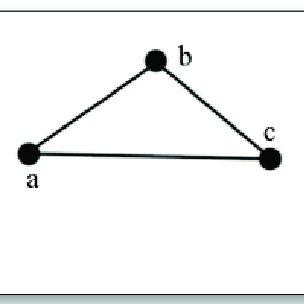
\includegraphics[scale=0.9]{nobip.jpg}

se representa como un archivo de texto como:\\
3 3\\
0 1\\
1 2\\
2 0\\

\begin{commandline}
\begin{verbatim}
  $ cat grafo.txt
  3 3
  0 1
  1 2
  2 0
  $ ./bip < grafo_1.txt
  El grafo de entrada no es bipartito.
\end{verbatim}
\end{commandline}

Se incluyen varios grafos ya representados como archivos de entrada:\\
núm vertices - num aristas\\
vertice origen - vertice destino\\
vertice origen - vertice destino\\
.. etc\\




\section{Referencias}
Introduction to Algorithms - 4th Edition Cormen Leiserson - Pág 563-565\\\\
Introduction to the Design \& Analysis of Algorithms - 3rd Edition - Levitin - Pág 29\\\\
Cápitulo 3 - Decomposición de grafos - Algorithms - S. Dasgupta\\\\
Intro DFS - \url{https://www.baeldung.com/cs/depth-first-search-intro}\\\\
The Vertex coloring problem and bipartite graphs \\ \url{https://tylermoore.ens.utulsa.edu/courses/cse3353/slides/l08-handout.pdf}\\\\
Bipartite Graphs - \url{https://www.geeksforgeeks.org/bipartite-graph/}\\\\
Learn DFS from scratch \\ \url{https://www.simplilearn.com/tutorials/data-structure-tutorial/dfs-algorithm#pseudocode_of_depthfirst_search_algorithm}\\\\
Bipartite graph Pág 3-7 \\ \url{https://speakerdeck.com/gustavoatt/bipartite-graph-matching-and-vertex-cover?slide=6}\\\\
Temas de C++ - \url{https://www.fing.edu.uy/tecnoinf/mvd/cursos/eda/material/teo/EDA-teorico14.pdf}\\\\
Array de vectores en C++ - \url{https://www.geeksforgeeks.org/array-of-vectors-in-c-stl/}\\\\
Vectores C++ - \url{https://www.programiz.com/cpp-programming/vectors}\\\\
Implementacion de un grafo para programacion competitiva \\ \url{https://www.geeksforgeeks.org/graph-implementation-using-stl-for-competitive-programming-set-1-dfs-of-unweighted-and-undirected/}

\end{document}

